% ON-THE-FLY
% explicar exploración parcial (lo visto hasta ahora)
% estados ganadores y perdedores ahora (antes era fácil, ahora tenemos que ver a dónde van)
% el concepto de ``frontera'' (en el sentido de transiciones existentes sin explorar) top, bottom
% actualizamos estado solo cuando estamos seguros (ganador en bottom / perdedor en top)
% exploramos de a una transición [e -l-> e']
% esto actualiza antecesores de e
% idea central de que ganador necesita loop


%dividimos en dos la explicación on-the-fly
%-------------------------------------------------------
\begin{frame}{Exploración parcial}
    La idea es intentar sacar conclusiones a medida que se explora, y construye a la vez, la composición total.
    
    Por ejemplo, en un momento dado podríamos tener explorado lo siguiente:
    \begin{figure}
     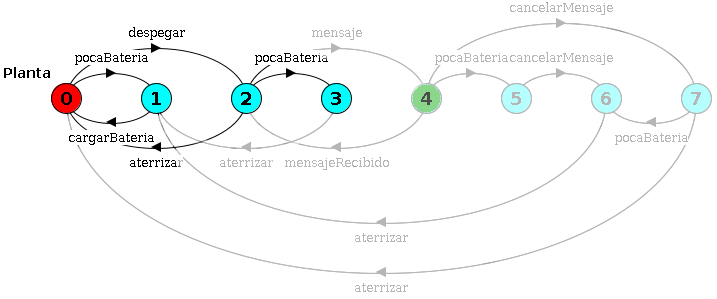
\includegraphics[width=\textwidth]{figures/partial.png}
    \end{figure}
    
    Exploramos de a una transición $e \step{\l}{} e'$ o paso.\vspace{10pt}\footnote{Los llamamos $e$ en vez de $t$ para resaltar que son \textit{estados de la planta}}
\end{frame}
%-------------------------------------------------------
\begin{frame}{Frontera optimista y pesimista}
    \begin{figure}
     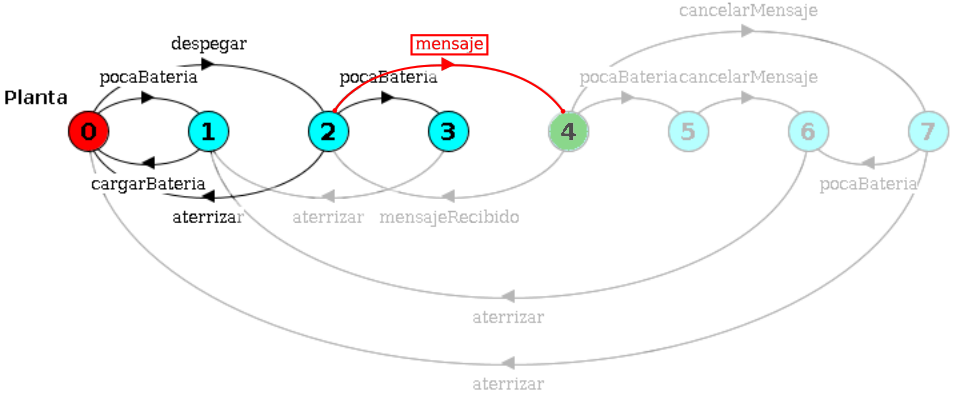
\includegraphics[width=\textwidth]{figures/frontera.png}
    \end{figure}
    El paso $2 \step{mensaje}{} 4$ está sin explorar. Como en principio no sabemos nada de él podríamos pensar que nos lleva a un estado ganador (frontera optimista) o perdedor (frontera pesimista).
\end{frame}
%-------------------------------------------------------
\begin{frame}{Nueva definición de ganadores/perdedores}
    En la versión monolítica es más simple reconocer ganadores/perdedores porque se cuenta con toda la información de la planta; en on-the-fly debemos ``imaginar'' a dónde van a parar las transiciones no vistas.
    
    Actualizamos estados sólo cuando estamos seguros, es decir, señalamos ganadores sólo al pensar una frontera pesimista y perdedores en frontera optimista.
    
    \begin{block}{Observación}
        Los estados ganadores/perdedores según esta definición son ganadores/perdedores en la planta completa, es decir, una vez que clasificamos un estado nunca debemos reconsiderarlo.
    \end{block}
\end{frame}
%------------------------------------------------------- %parte 2
\begin{frame}{Propagar información}
	Si estamos explorando una transición nueva $e \step{\l}{} e'$:
	
	\pause
	
	Un estado $s$ es un \textbf{nuevo} ganador/perdedor si: sin explorar la última transición no teníamos suficiente información y ahora sí.
	
	\pause
	
	$s$ solo tiene nueva información si \textbf{puede alcanzar} la nueva transición. ($s$ tiene que ser un antecesor de $e$).
	
	\pause 
	
	si no sabemos si $e'$ gana o pierde, no tenemos información para propagar, porque \textbf{la transición nueva va a lo desconocido}.

\end{frame}
%-------------------------------------------------------
\begin{frame}{Obtener nueva información (Ganador)}
	Como vimos, queremos trazas que visiten \textbf{infinitas} veces un estado marcado. \pause Una traza infinita en un autómata finito solo puede ocurrir si forma un \textbf{ciclo} (loop).
	
	\pause
		
	Ese ciclo debe tener un \textbf{estado marcado} o previamente \textbf{clasificado ganador}.
	
	\pause
	
	Al explorar una nueva transición ($e \step{\l}{} e'$), en el caso que $e'$ no esté clasificado, analizamos el ciclo \textbf{mas grande} que forma. Si no podemos ganar en ese ciclo, no obtuvimos nuevos ganadores.
	
	\pause

	Para ganar el ciclo debe ser \textbf{controlablemente cerrado}. Intuición: Si una transición no controlable sale del ciclo, un controlador no puede mantenerse ahí dentro y ganar. Y si por no mantenerse adentro, va a un estado no explorado, \textbf{somos pesimistas} y asumimos que pierde.
\end{frame}
%-------------------------------------------------------
\begin{frame}{Obtener nueva información (Perdedor)}
	Descubrimos nuevos estados perdedores cuando \textbf{seguro} sabemos que no forman trazas con infinitos estados marcados.
	
	\pause 
	
	Esto es obvio cuando el estado solo tiene la traza vacía. \textbf{No puede ir a ningún otro estado}.
	
	\pause 
	
	Más difícil de detectar son los \textbf{ciclos sin estados marcados}.
	
	\pause
	
	\begin{block}{caso general}
		Si en todos los descendientes de un estado $e$, no hay ningún \textbf{ciclo ganador}, entonces $e$ tiene que ser perdedor. 
		
		Tenemos que chequear \textbf{todos} los descendientes, porque siendo \textbf{optimistas}, un descendiente desconocido podría ser ganador.
	\end{block}
	
	%acá decir que en la posta es + dificil xq podes tener un descendiente que sea ganador pero sos perdedor xq se te propaga perdedor de otro descendiente que no podes evitar, pero que esta es la forma de detectar "nuevos" perdedores.
\end{frame}
%-------------------------------------------------------
\begin{frame}{Resúmen del nuevo algoritmo}
    \begin{itemize}
     \item Clasificamos (ganador/perdedor) cuando estamos seguros. %i.e. no se cambia una vez que está
     \item Propagamos a los antecesores afectados (si hay información respecto a e').
     \item Tratamos de obtener nueva información sólo al cerrar loops.
    \end{itemize}
    
    \begin{block}{Observación:}
        Sólo hacemos nuevos cálculos cuando son realmente necesarios.
    \end{block}
    
    Nos interesa saber qué tan buena es la eficiencia del algoritmo, en tiempo de cómputo.
\end{frame}


